% 
% chapter6.tex
% ThesisISEL
% 
% Created by Serge Lage on 2019/09/30.
%
% ================
% = Validation =
% ================
\chapter{Validation}
\label{cha:validation}

This chapter describes the process used to evaluate the work done in this thesis.

\section{Validation of Standalone Fishery Analysis} % (fold)
\label{sec:val_SFA}

The VMS data are not classified, for the validation and evaluation of SFALib presented in chapter \ref{cha:standalone_fishery_analysis}, the first step consists in the classification of the data.

The classification is realized using three categories, as follows:
\begin{itemize}
\item Class 0 = Fishing in a known area;
\item Class 1 = Not Fishing;
\item Class 2 = Fishing in a new area.
\end{itemize} 


It was chosen the vessel with id two because it has the most entries in the database provided to this work. In Figure \ref{fig:bi_2_all}, the circles represent locations given by the VMS data to vessel two, and the size of the circle, the velocity. This analysis was done using Windows Power Bi \cite{WEBSITE:PowerBi}.

\begin{figure}[]
\centering
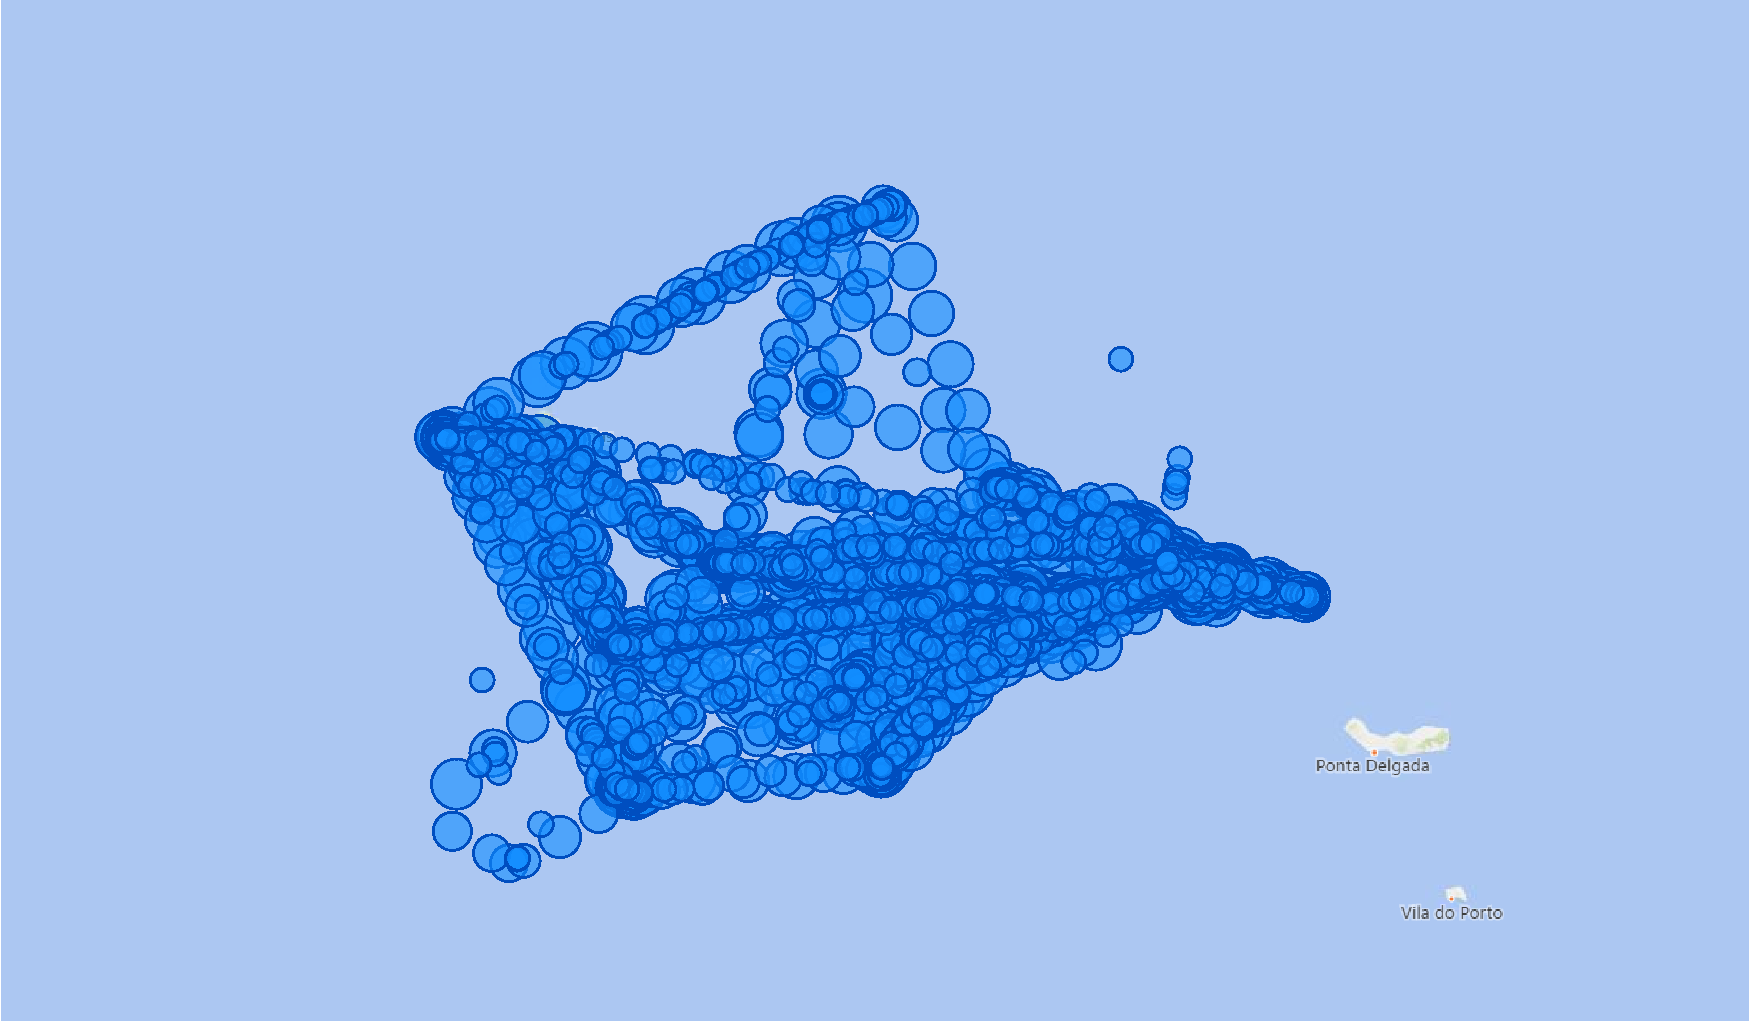
\includegraphics[width=0.8\linewidth]{Chapters/img/2All.pdf}
\caption{Representation of all VMS coordinates for vessel 2 }
\label{fig:bi_2_all}
\end{figure}
\newpage
To get data to test SFALib, we need to classify data into three classes.
\begin{itemize}
\item Class 0 (Fishing in a known area): To get data to classify as fishing in an area, the data was filtered with a SOG between 0 and 4. Number 4 was chosen because of the analysis made in chapter 3.3, which concludes that the fishing activity done by this vessel is at speeds below four nautical miles. With this, we end up with the data represented in Figure \ref{fig:bi_2_all}. To extract the text data, it was chosen the fishing spot near the island of Flores represented in Figure \ref{fig:bi_2_flores}. 500 random VMS entries were collected at this location without speed restriction. This means that we may have collected travel data, but no speed bias was passed to this test data. 


\begin{figure}[]
\centering
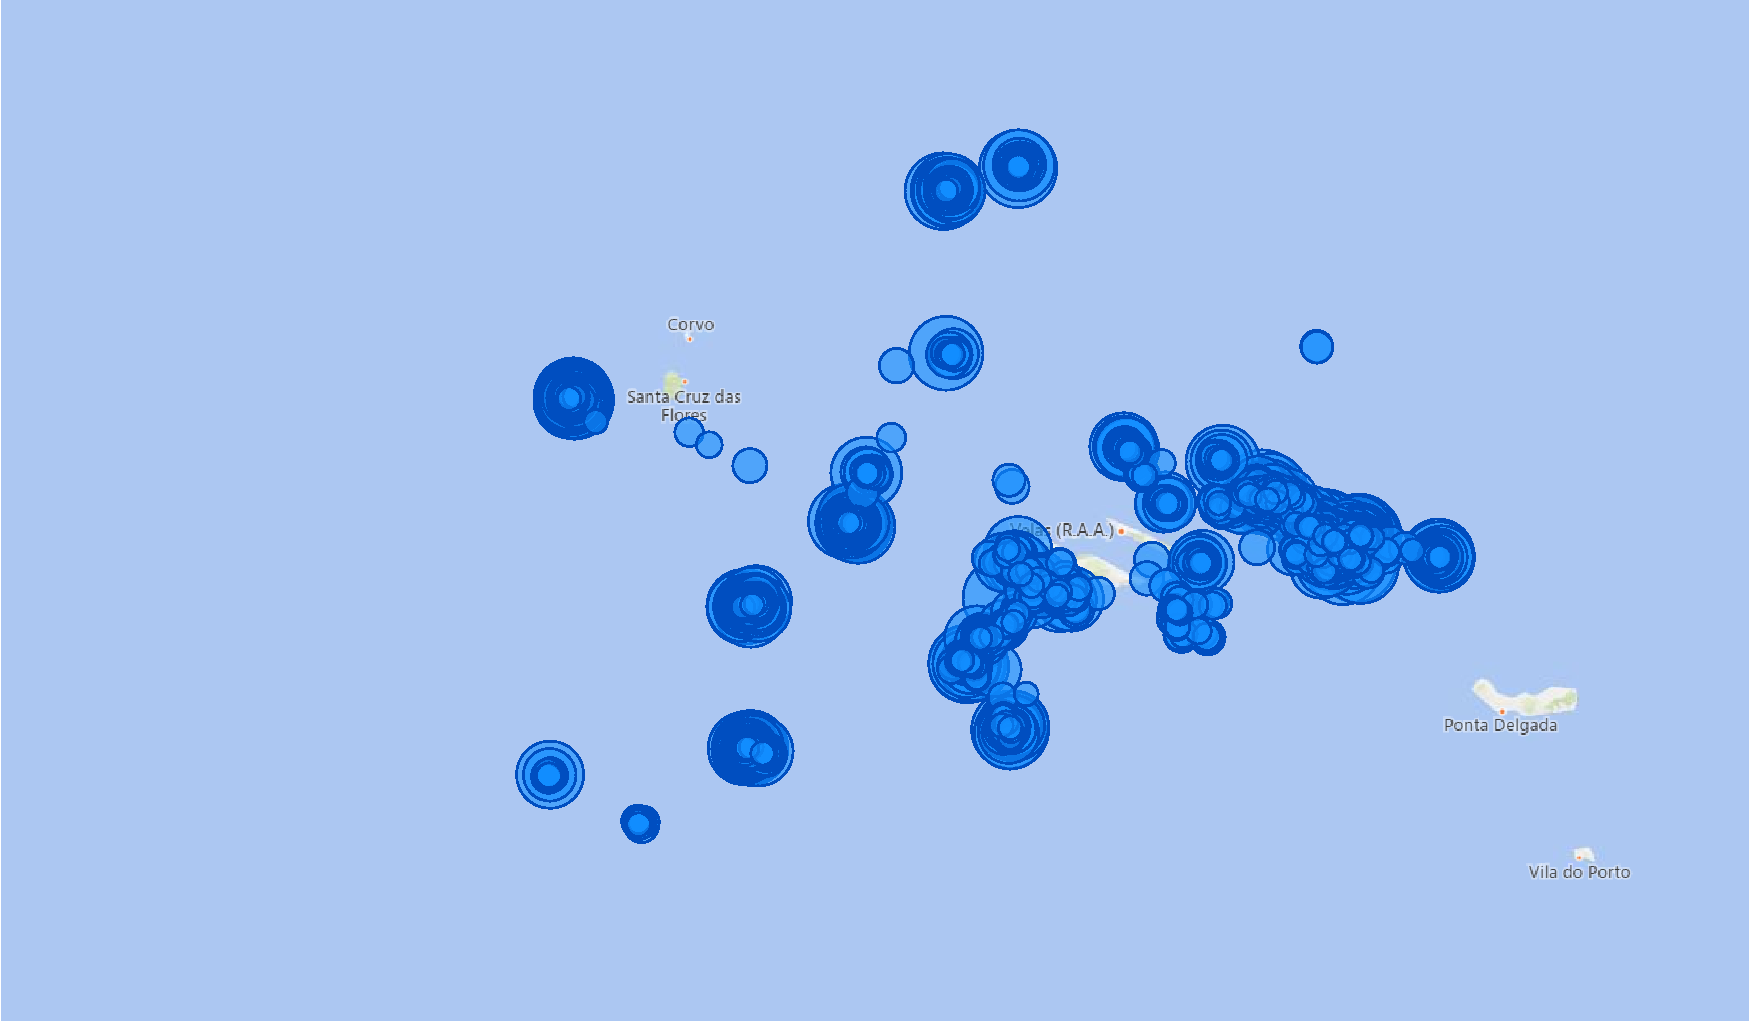
\includegraphics[width=0.8\linewidth]{Chapters/img/2fishingAll.pdf}
\caption{Representation of VMS coordinates for vessel 2 with speeds inferior of 4 }
\label{fig:bi_2_all}
\end{figure}

\begin{figure}[]
\centering
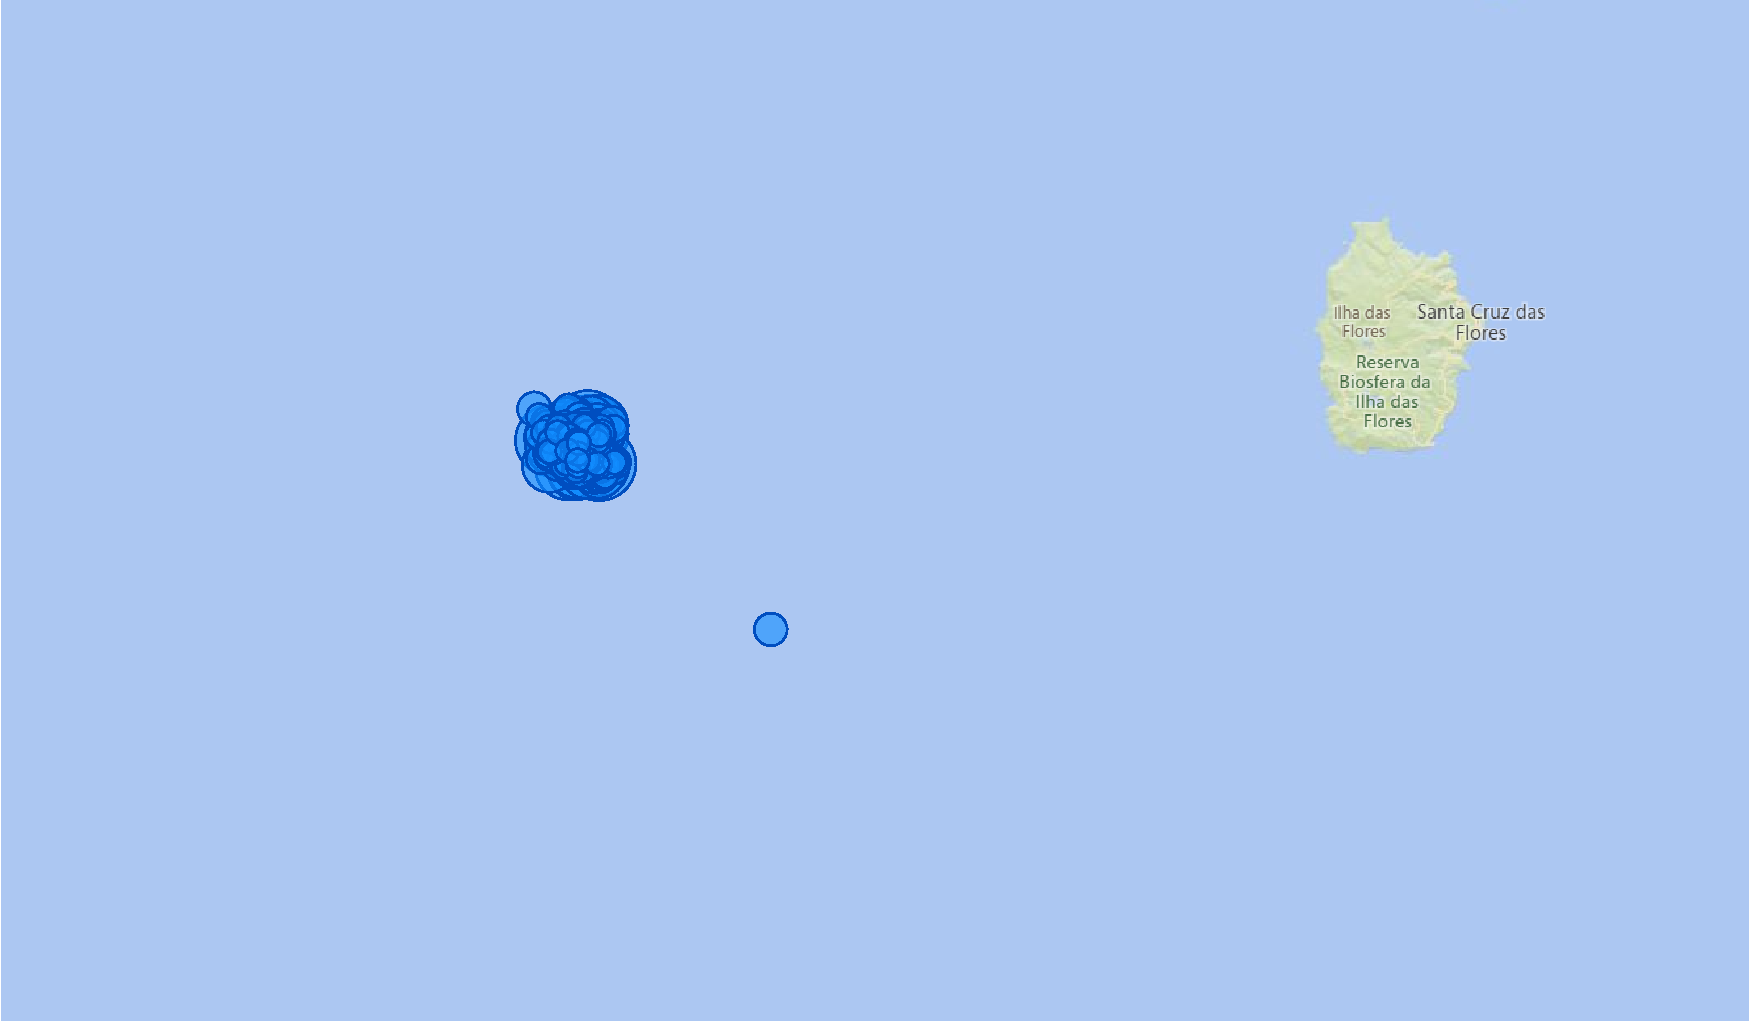
\includegraphics[width=0.8\linewidth]{Chapters/img/2fishing.pdf}
\caption{Representation of VMS coordinates for vessel 2 with speeds inferior of 4 near Flores island }
\label{fig:bi_2_flores}
\end{figure}

\item Class 1 (Not fishing): For with class, it was extracted 500 random VMS entries with the location near Terceira island represented in figure \ref{fig:bi_2_travel}. It was chosen this spot because most points appear to be on a well-defined trajectory. This pattern contrasts with the random-looking and under-lapping points in Figure \ref{fig:bi_2_flores}. 

\begin{figure}[]
\centering
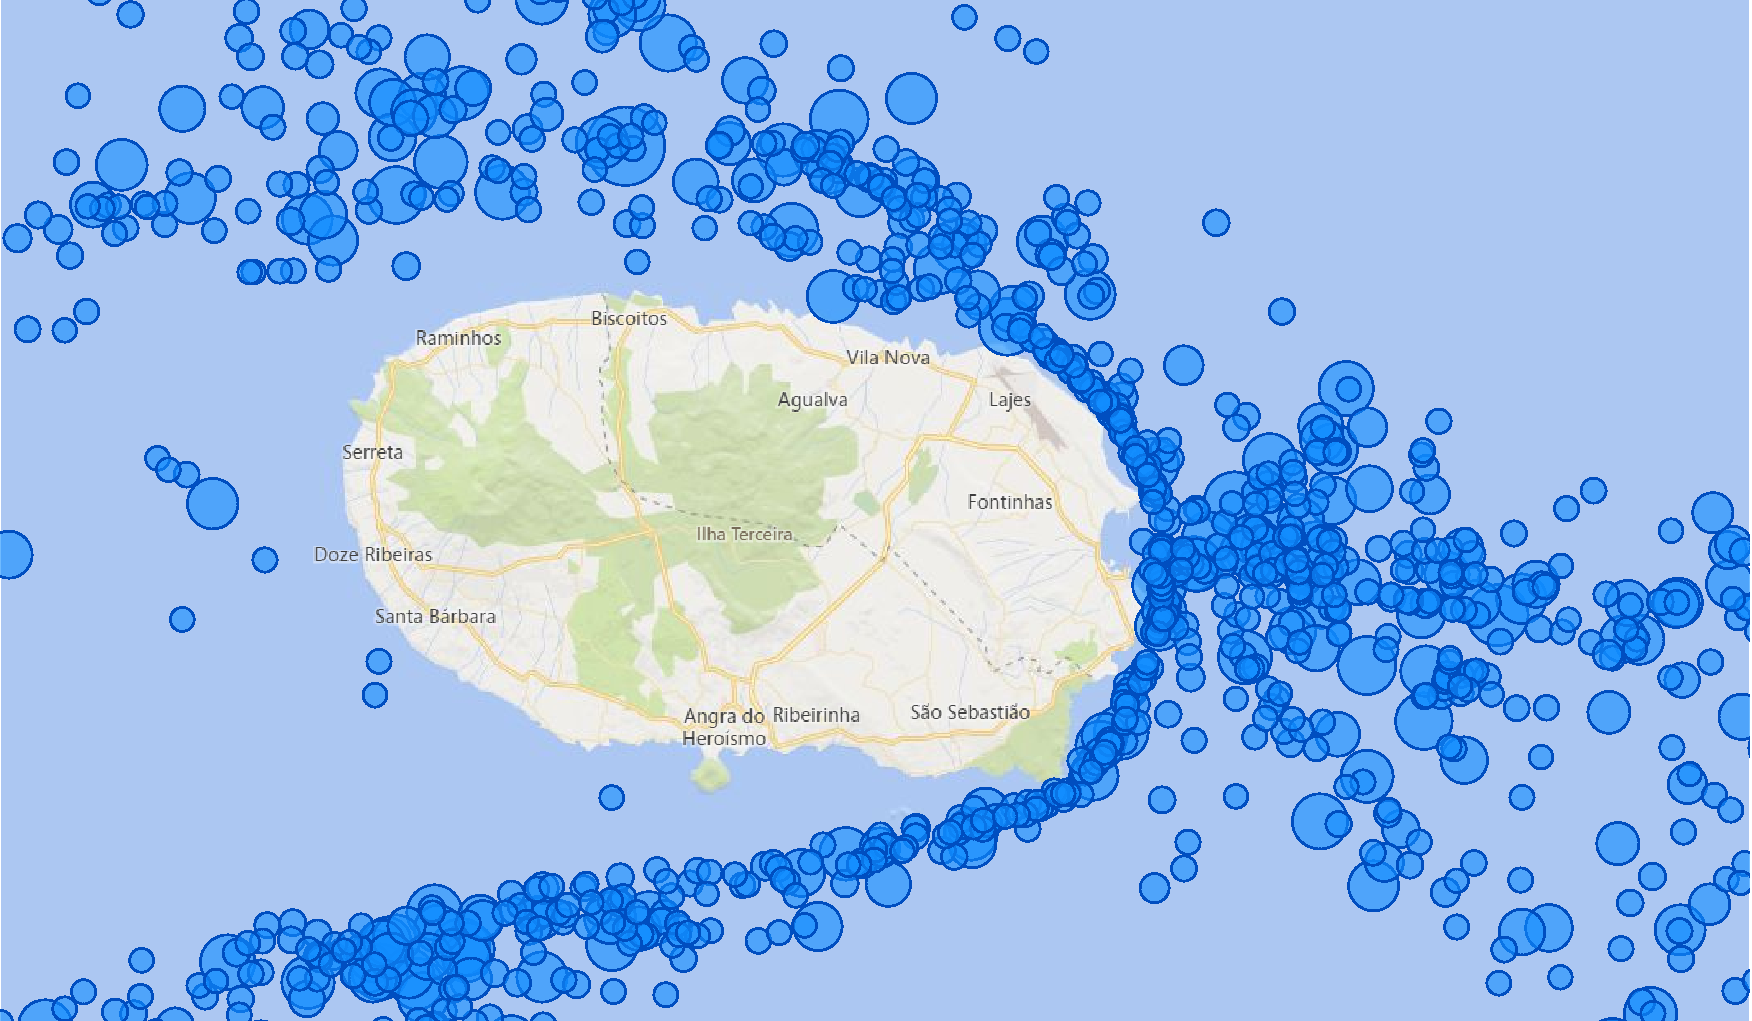
\includegraphics[width=0.8\linewidth]{Chapters/img/2viagem.pdf}
\caption{Representation of VMS coordinates for vessel 2 near Terceira island}
\label{fig:bi_2_travel}
\end{figure}



\item Class 2 (Fishing in a new area): To have data from this class, it was created new data. So 500 new VMS entries were created. The data was created using the data from class 0 but changing to a location near mainland Portugal that is placed with no entries for with vessel. 

\end{itemize}




\subsection{Validation and evaluation}
\label{sec:val_SFA_val_eva}

To evaluate the classification accuracy of SFALib, it was used precision and recall.

\textbf{Precision:} Proportion of positive identifications that was actually correct is measured as \(\frac{tp}{tp+fp} \).\\
In table \ref{table:val_sfa_pr} we can see that the lower the configuration value for velocity, the better are the results.
This can mean that the gap in speed between fishing and traveling is big.

The best result has an average precision of 0.9.


\begin {table}[H]
\begin{center}
\begin{tabular}{c|c|c|c}
Configuration for velocity & \textbf{Fishing} & \textbf{No Fishing} & \textbf{Fishing in new area} \\\hline
0.1 & 0.67 & 1 & 0.67 \\
0.05 & 0.738 & 1 & 0.738 \\
0.01 & 0.838 & 1 & 0.838 \\
0.001 & 0.85 & 1 & 0.85 \\
0 & 0.85 & 1 & 0.85 
\label{table:val_sfa_pr}
\end{tabular}
\caption {Precision per class per configuration}
\end{center}
\end {table}


\textbf{Recall:} Proportion of actual positives that was identified correctly is measured as \(\frac{tp}{tp+fn} \). \\
In Table \ref{table:val_sfa_re} we can confirm that, like in precision, the recall is better with a low configuration value for velocity.

The best result has an average recall of 0.9231.

\begin {table}[H]
\begin{center}
\begin{tabular}{c|c|c|c}
Configuration for velocity & \textbf{Fishing} & \textbf{No Fishing} & \textbf{Fishing in new area} \\\hline
0.1 & 1 & 0.6024 & 1 \\
0.05 & 1 & 0.6562 & 1 \\
0.01 & 1 & 0.7553 & 1 \\
0.001 &1 & 0.7692 & 1 \\
0 &1 & 0.7692 & 1
\label{table:val_sfa_re}
\end{tabular}
\caption {Recall per class per configuration}
\end{center}
\end {table}

In Table \ref{table:val_sfa_cm}, we can see that there is some fishing and fishing classified data that was predicted as not fishing. However, considering that the classified data can have some errors in classification, we cannot assure that the predicted not fishing of fishing classed is not actually, not fishing. 

\begin {table}[H]
\begin{center}
\begin{tabular}{c|c|c|c}
Prediction/Real & \textbf{Fishing} & \textbf{No Fishing} & \textbf{Fishing in new area} \\\hline
Fishing & 0.85 & 0 & 0 \\
No Fishing & 0.15 & 1 & 0.15 \\
Fishing in new area & 0 & 0 & 0.85 
\label{table:val_sfa_cm}
\end{tabular}
\caption {Confusion matrix for configuration with 0.001 for velocity}
\end{center}
\end {table}


% section val_SFA (end)

\section{Validation of Joined Fishery Analysis} % (fold)
\label{sub:val_JFA}

To validate and evaluation of the model used for Joined Fishery Analysis decided in subsection \ref{sub:evaluation} as being Random Forest, it was used the same data as in subsection \ref{sub:evaluation}.

In subsection \ref{sub:evaluation} we use cross-validation \cite{CrossValidatory} that trains the model with approximately the same percentage of samples of each target class as the complete set.
In this validation, it was only used one vessel of each license for the train and all of the tests. In this case, we will train the model with 11 vessels but test with 30. This model will have a strong bias to these 11 vessels, but we will see the degradation of the results when testing with these unknown vessels by the model.
This is useful to understand the importance of having the model up to date and how badly it preforms with new vessels. 





\subsection{Validation and evaluation}
\label{sec:val_JFA_val_eva}
% section val_JFA (end)
To evaluate the classification accuracy of Joined Fishery Analysis model it was used a confusion matrix and the model precision and recall.

In figure \ref{fig:val_jfa} we can observe that this model is less accurate that the model tested in Figure \ref{fig:cm_rf}. 
The precision in this model is 0.6727, and the recall is 0.6379.

This means that different vessels in the same license can operate at different speeds, and so for the model to work without differentiation of vessel power, length, or gross tonnage, it requires that the training dataset is varied in the type of vessels.
The other solution is to create different models by categorizing vessels by vessel information(Gross tonnage, length, and power). This way, the models can by specific and achieve better results. 

\begin{figure}[H]
\centering
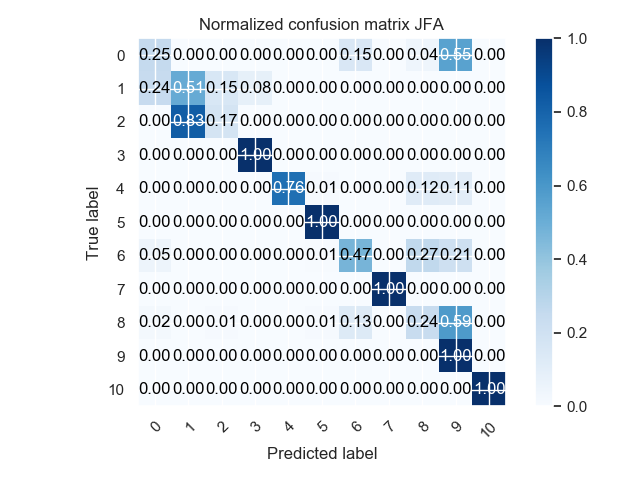
\includegraphics[width=0.8\linewidth]{Chapters/img/val_JFA.png}
\caption{Confusion Matrix for Joined Fishery Analysis validation }
\label{fig:val_jfa}
\end{figure}



% chapter conclusion (end)


